\documentclass[10pt]{article}
\usepackage[utf8]{inputenc}
\usepackage[T1]{fontenc}
\usepackage{graphicx}
\usepackage[export]{adjustbox}
\graphicspath{ {./images/} }

\title{Bachelor of Science (BSc) in Informatik Modul Software-Entwicklung 1 (SWEN1) }

\author{}
\date{}


\begin{document}
\maketitle
\section*{LE 02 - Anforderungsanalyse I}
\section*{SWEN1/PM3 Team}
R. Ferri (feit), D. Liebhart (lieh), K. Bleisch (bles), G. Wyder (wydg)

\section*{Warm-Up}
\begin{itemize}
  \item Wenn Sie nur drei Wünsche (Forderungen) an eine Software, die Sie verwenden, stellen könnten:
  \item Was wären Ihre drei Forderungen?
  \item Zeit: 3 Minuten
\end{itemize}

\section*{Um was geht es?}
\begin{itemize}
  \item Wie findet man die wichtigen Anforderungen an ein Softwareprodukt?
  \item Was ist Usability und wieso ist das wichtig für die Softwareentwicklung?
\end{itemize}

\section*{Lernziele LE 02 - Anforderungsanalyse I}
Sie sind in der Lage,

\begin{itemize}
  \item die wichtigsten Begriffe des Usability-Engineering zu nennen.
  \item die wichtigsten Usability-Anforderungen zu erläutern.
  \item das Vorgehen des User-Centered Designs zu skizzieren.
  \item die wichtigsten Ziele, Methoden und Artefakte der einzeInen Phasen des UCD zu erklären.
  \item ein einfaches Geschäftsprozessmodell zu interpretieren.
\end{itemize}

\section*{1. Was ist Usability}
\begin{enumerate}
  \setcounter{enumi}{1}
  \item Was sind die wichtigsten Usability-Anforderungen
  \item Wie kann man diese Forderungen bei der Softwareentwicklung umsetzen
  \item Wrap-up und Ausblick
\end{enumerate}

\section*{Usability}
School of\\
Engineering InIT Institut für angewandte Informationstechnologie

\begin{itemize}
  \item Usability: Definition gemäss DIN ISO 9241
\end{itemize}

Die Effektivität, Effizienz und Zufriedenheit\\
mit der die adressierten Benutzer ihre Ziele erreichen in ihren spezifischen Kontexten.

\begin{itemize}
  \item 4 wichtige Aspekte
  \item Benutzer
  \item Seine Ziele/Aufgaben
  \item Sein Kontext
  \item Softwaresystem (inkl. UI)\\
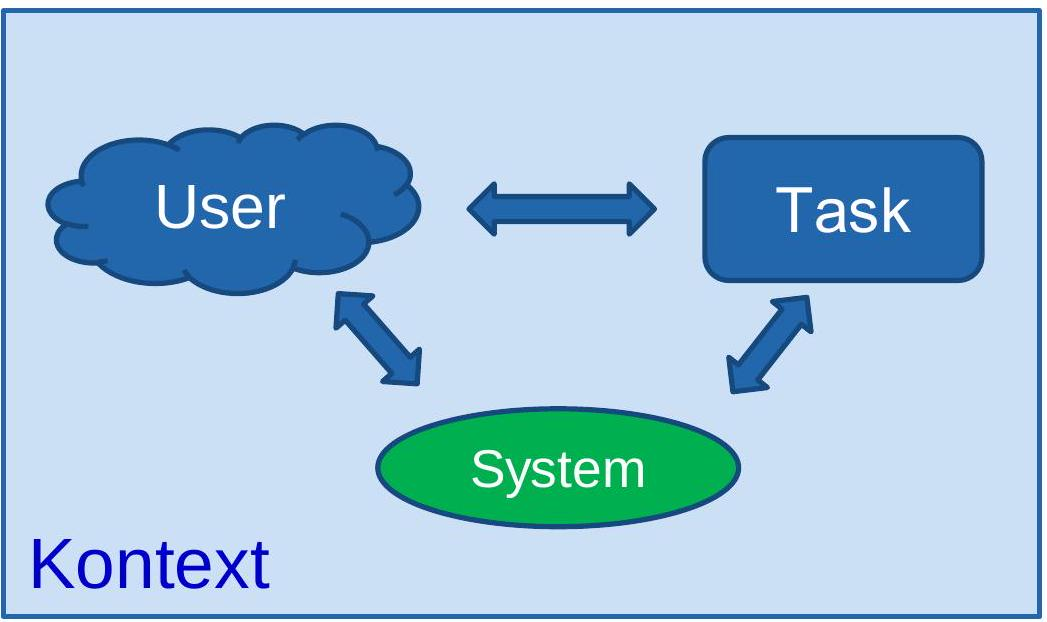
\includegraphics[max width=\textwidth, center]{2025_01_02_6e0302462f81f53e08d0g-06}
\end{itemize}

\begin{enumerate}
  \item Was ist Usability
  \item Was sind die wichtigsten Usability-Anforderungen
  \item Wie kann man diese Forderungen bei der Softwareentwicklung umsetzen
  \item Wrap-up und Ausblick
\end{enumerate}

\begin{itemize}
  \item 7 wichtige Anforderungsbereiche bezüglich Usability
  \item Aufgabenangemessenheit
  \item Lernförderlichkeit
  \item Individualisierbarkeit
  \item Erwartungskonformität
  \item Selbstbeschreibungsfähigkeit
  \item Steuerbarkeit
  \item Fehlertoleranz
\end{itemize}

\begin{enumerate}
  \item Was ist Usability
  \item Was sind die wichtigsten Usability-Anforderungen
  \item Wie kann man diese Forderungen bei der Softwareentwicklung umsetzen
  \item Wrap-up und Ausblick
\end{enumerate}

\section*{User-Centered Design}
\begin{itemize}
  \item Berücksichtigt die Bedürfnisse, Wünsche, Einschränkungen der Benutzer in jeder Phase des DesignProzesses
  \item UCD Process (ISO 9241)\\
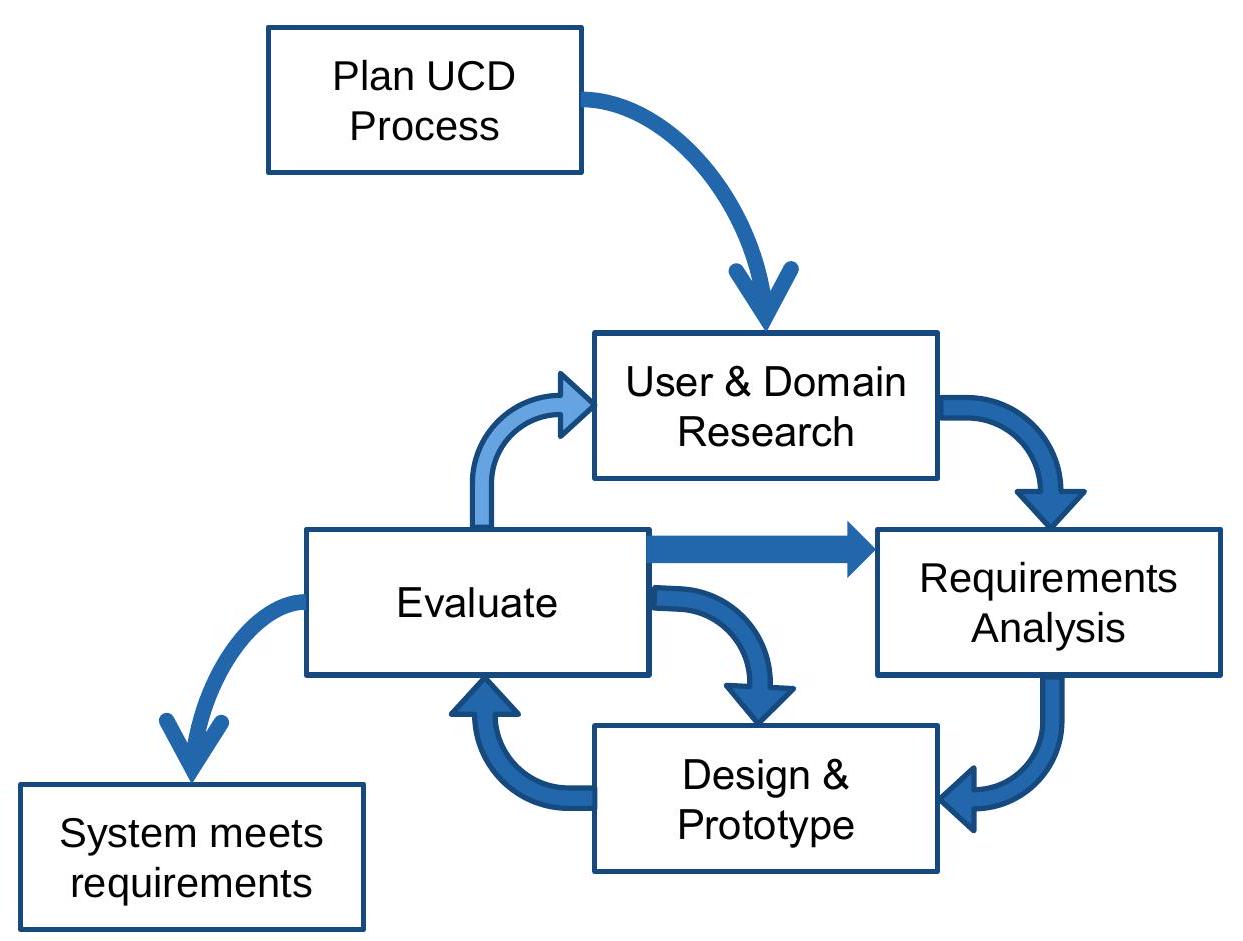
\includegraphics[max width=\textwidth, center]{2025_01_02_6e0302462f81f53e08d0g-10}
\end{itemize}

\section*{UCD Process \\
 User \& Domain Research}
\begin{itemize}
  \item Ziele bezüglich User
  \item Wer sind die Benutzer?
  \item Was ist ihre Arbeit, ihre Aufgaben, Ziele?\\
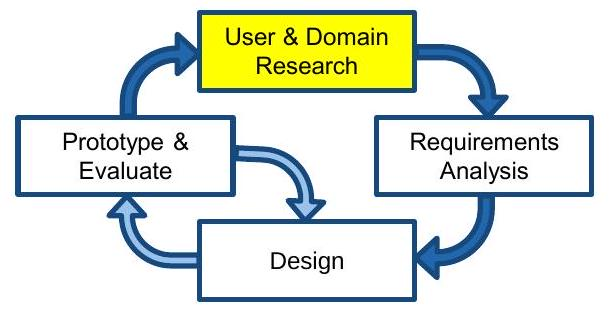
\includegraphics[max width=\textwidth, center]{2025_01_02_6e0302462f81f53e08d0g-11}
  \item Wie sieht ihre (Arbeits-)Umgebung aus?
  \item Was brauchen sie, um ihre Ziele zu erreichen?
  \item Welche Sprache sprechen sie, welche Begriffe verwenden sie?
  \item Welche Normen sind wichtig für sie (organisatorisch, kulturell, sozial)
  \item Pain Points in ihrer Arbeit (Brüche, Workarounds)
\end{itemize}

\section*{UCD Process \\
 User \& Domain Research}
\begin{itemize}
  \item Hauptziele bezüglich Domäne
  \item Business der Firma verstehen
  \item Domäne verstehen\\
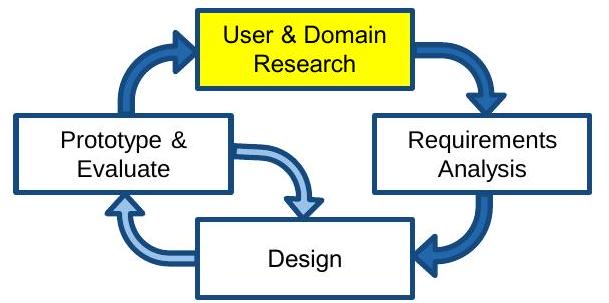
\includegraphics[max width=\textwidth, center]{2025_01_02_6e0302462f81f53e08d0g-12}
  \item Sprache
  \item Wichtigste Konzepte
  \item Prozesse
\end{itemize}

\section*{UCD Process \\
 User \& Domain Research}
\begin{itemize}
  \item Methoden des User \& Domain Research
  \item Contextual Inquiry
  \item Interviews\\
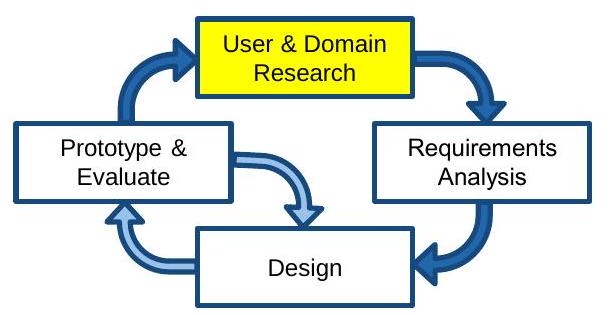
\includegraphics[max width=\textwidth, center]{2025_01_02_6e0302462f81f53e08d0g-13}
  \item Beobachtung
  \item Fokusgruppen
  \item Umfragen
  \item Nutzungsauswertung
  \item Desktop Research
  \item Dokumentenstudium
  \item Mitbewerber\\
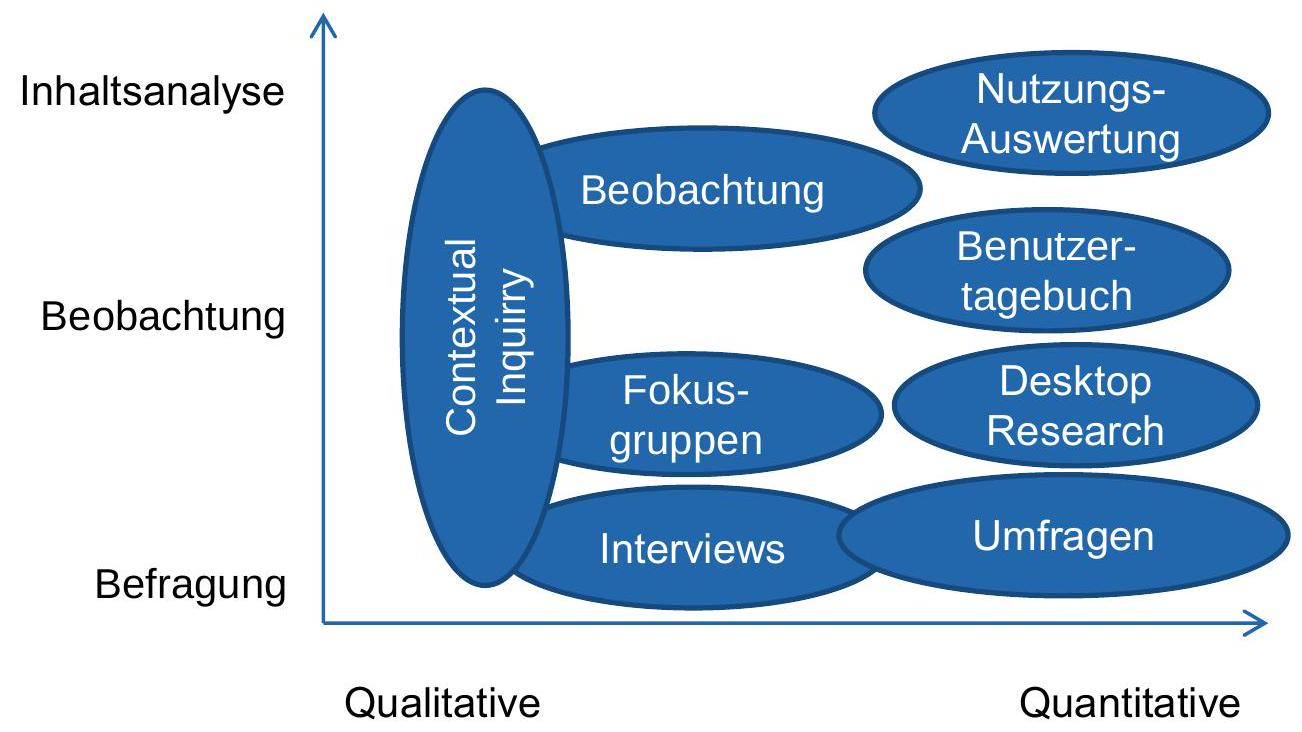
\includegraphics[max width=\textwidth, center]{2025_01_02_6e0302462f81f53e08d0g-13(1)}
\end{itemize}

\section*{User \& Domain Research Wichtige Artefakte}
\begin{itemize}
  \item Personas
  \item Usage-Szenarien
  \item Mentales Modell\\
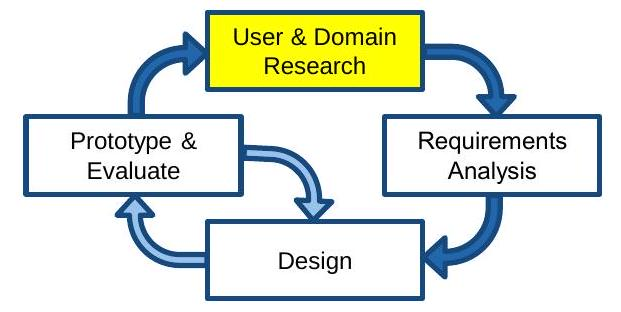
\includegraphics[max width=\textwidth, center]{2025_01_02_6e0302462f81f53e08d0g-14}
  \item Domänenmodell
  \item Stakeholder Map
  \item Service Blueprint / Geschäftsprozessmodell
\end{itemize}

\section*{User \& Domain Research Artefakte Persona}
School of Engineering InIT Institut für angewandte Informationstechnologie

\begin{itemize}
  \item Eine fiktive Person
  \item Repräsentiert eine bestimmte Benutzergruppe
  \item Mit gleichem Verhalten, Bedürfnissen, Interessen
  \item In einer bestimmten Rolle
  \item Wichtig, um Design-Entscheide zu diskutieren und kommunizieren\\
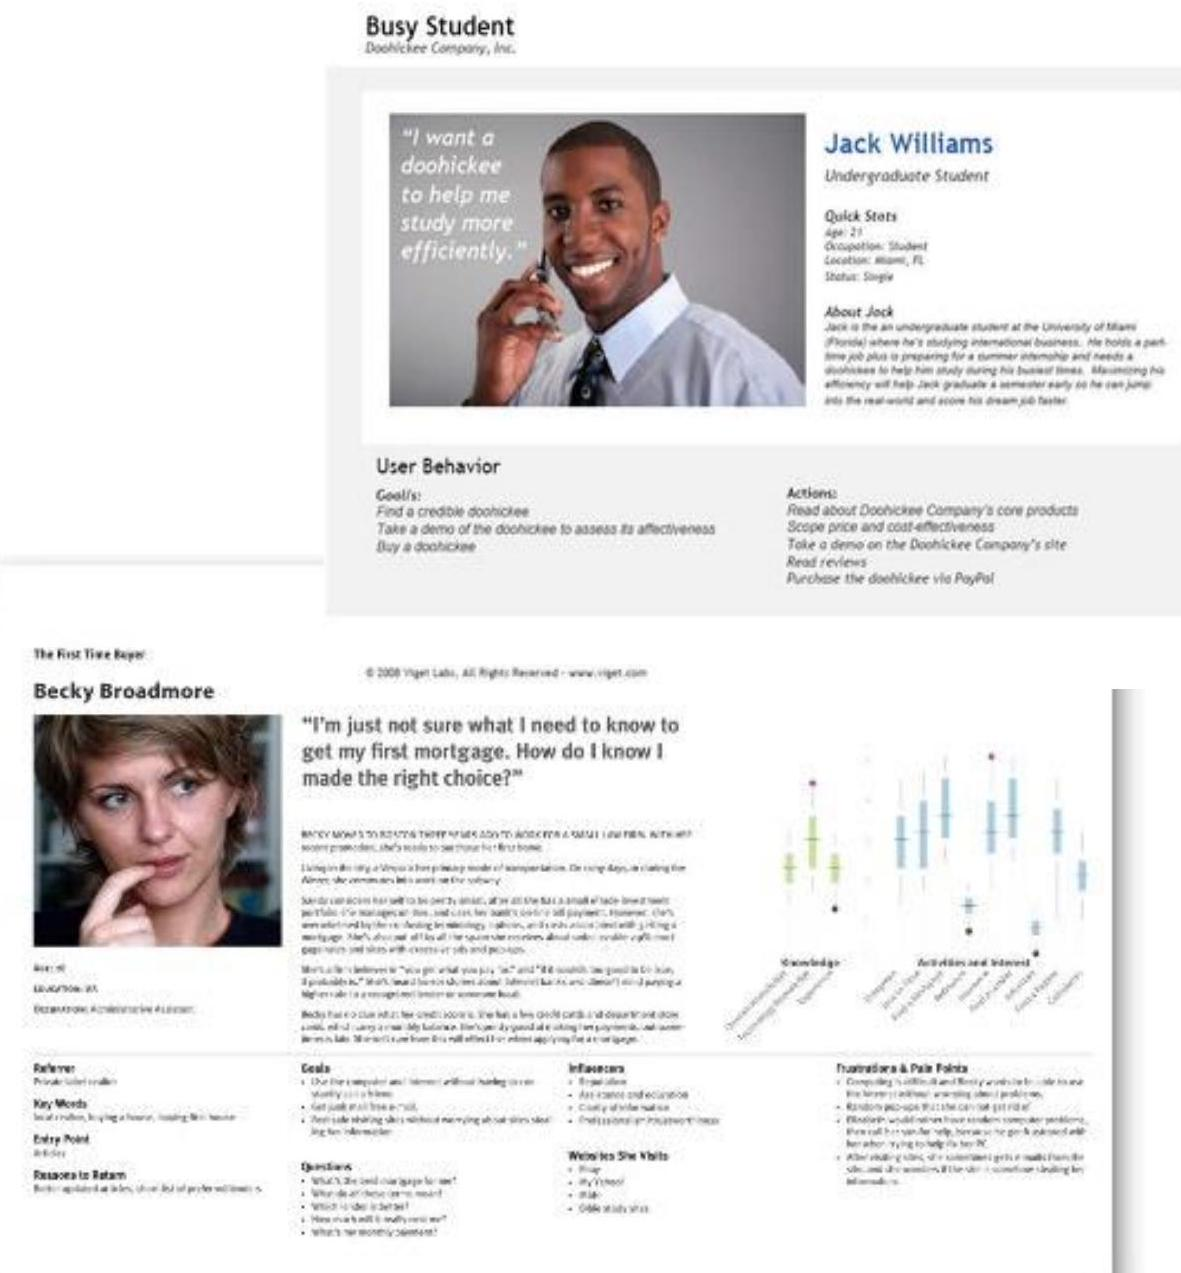
\includegraphics[max width=\textwidth, center]{2025_01_02_6e0302462f81f53e08d0g-15}
\end{itemize}

\section*{User \& Domain Research Wichtige Artefakte}
\begin{itemize}
  \item Personas
  \item Usage-Szenarien
  \item Mentales Modell
  \item Domänenmodell
  \item Stakeholder Map
  \item Service Blueprint / Geschäftsprozessmodell
\end{itemize}

\section*{User \& Domain Research Artefakte Szenarien}
\begin{itemize}
  \item Szenarien im UCD
  \item Kurze Geschichte, wie ein Benutzer (Persona) ein (Software-) Produkt in einer konkreten Situation benützt, um eine bestimmte Aufgabe (Job) zu erledigen.
  \item 2 Arten von Szenarien wichtig
  \item Usage-Szenarien
  \item Beschreiben die aktuelle Situation
  \item Werden vor allem in der User \& Domain Research verwendet
  \item Kontextszenarien
  \item Beschreiben die zukünftige gewünschte Situation
  \item Werden vor allem in der Anforderungsanalyse des UCD verwendet
\end{itemize}

\section*{User \& Domain Research Wichtige Artefakte}
School of Engineering InIT Institut für angewandte Informationstechnologie

\begin{itemize}
  \item Personas
  \item Usage-Szenarien
  \item Mentales Modell
  \item Stakeholder Map
  \item Service Blueprint / Geschäftsprozessmodell
  \item Stakeholder Map
  \item Zeigt die wichtigsten Stakeholder im Umfeld der Problemdomäne\\
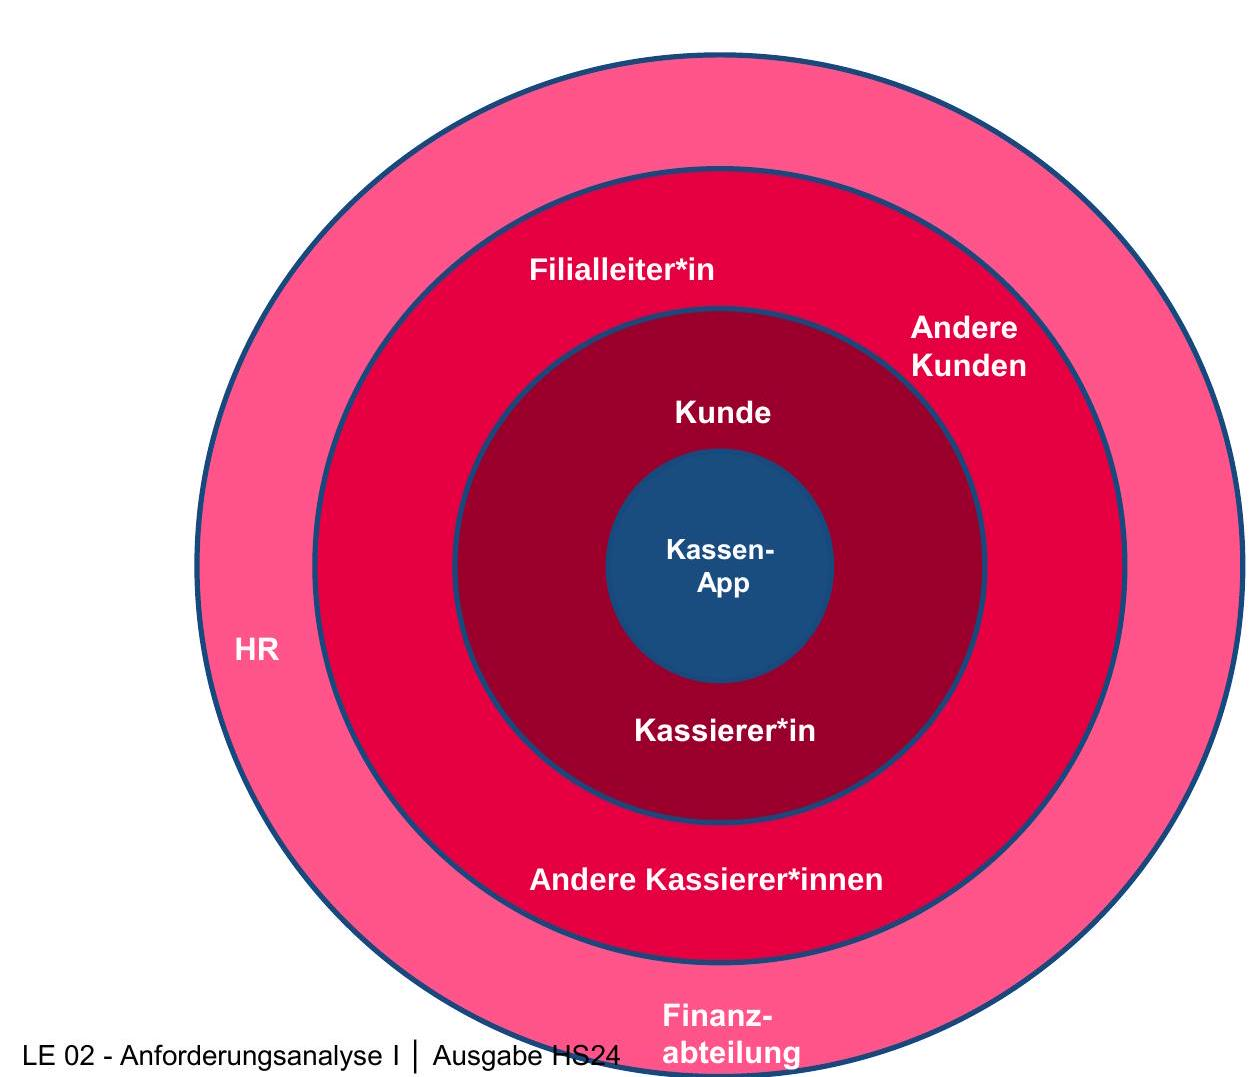
\includegraphics[max width=\textwidth, center]{2025_01_02_6e0302462f81f53e08d0g-18}
\end{itemize}

\section*{User \& Domain Research Wichtige Artefakte}
\begin{itemize}
  \item Personas
  \item Usage-Szenarien
  \item Mentales Modell
  \item Stakeholder Map
  \item Service Blueprint / Geschäftsprozessmodell
  \item Bespiel: Doodle-Service\\
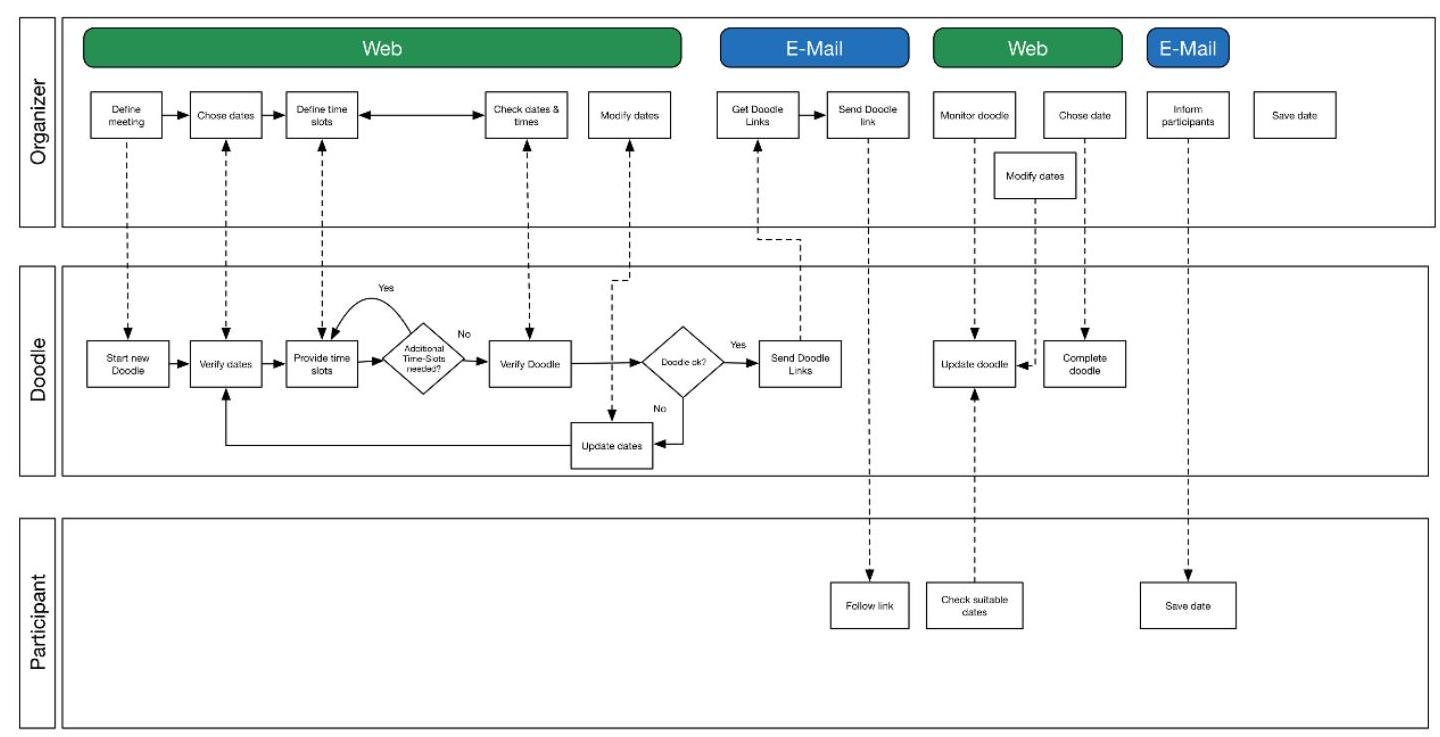
\includegraphics[max width=\textwidth, center]{2025_01_02_6e0302462f81f53e08d0g-19}
\end{itemize}

\section*{Weitere wichtige Artefakte aus dem UCD}
\begin{itemize}
  \item UI-Skizzen
  \item (Hand-) Skizzen der wichtigsten Screens, die für ein Kontextszenario notwendig sind
  \item Wireframes
  \item UI-Prototypen (Low-Fidelity, High-Fidelity), die das Interaktionskonzept demonstrieren
  \item Werden auch für die Evaluation des Interaktionskonzepts mit Usern eingesetzt
  \item Weitere Usability-Anforderungen
  \item UI-Designs
  \item Vorlagen für die UI-Umsetzung
\end{itemize}

\section*{UCD Prozess \\
 Anforderungsanalyse}
\begin{itemize}
  \item Ausgehend von den Resultaten des UCD
\end{itemize}

User-Anforderungen an das zu entwickeInde System ableiten\\
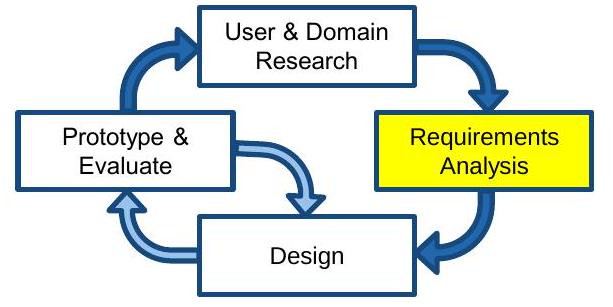
\includegraphics[max width=\textwidth, center]{2025_01_02_6e0302462f81f53e08d0g-21}

\begin{itemize}
  \item Funktionale Abläufe, Interaktionen:
  \item Kontextszenarien, Storyboards, Ul-Skizzen, Use Cases
  \item Konzepte, Beziehungen, Quantitäten:
  \item Domänenmodell
  \item Weitere funktionale/nicht-funktionale Anforderungen, Randbedingungen:
  \item FURPS-Modell (Functionality, Usability, Reliability, Performance, Supportability)
\end{itemize}

\section*{UCD Anforderungsanalyse: Artefakte Kontextszenario}
\begin{itemize}
  \item Beschreibt die zukünftige, gewünschte Situation
  \item Wie der Benutzer seinen Job mit der zünftigen Lösung erledigt
  \item Beschreibung aus Benutzersicht
  \item Interaktionsschritte mit dem System
  \item High Level, ohne konkrete UI-Lösungskonzepte
  \item Beschreiben den Kontext für die späteren Use Cases
\end{itemize}

\section*{User \& Domain Research Artefakte Storyboard}
\begin{itemize}
  \item Visualisiert Kontextszenario als Comic
  \item 6-8 Bilder mit 1-2 Sätzen Beschreibung
  \item Von Hand skizziert
  \item Storyboarding-Tools verfügbar
  \item Zeigt:
  \item Schlüsselszenen des Szenarios
  \item Wichtigste Ideen, Screens\\
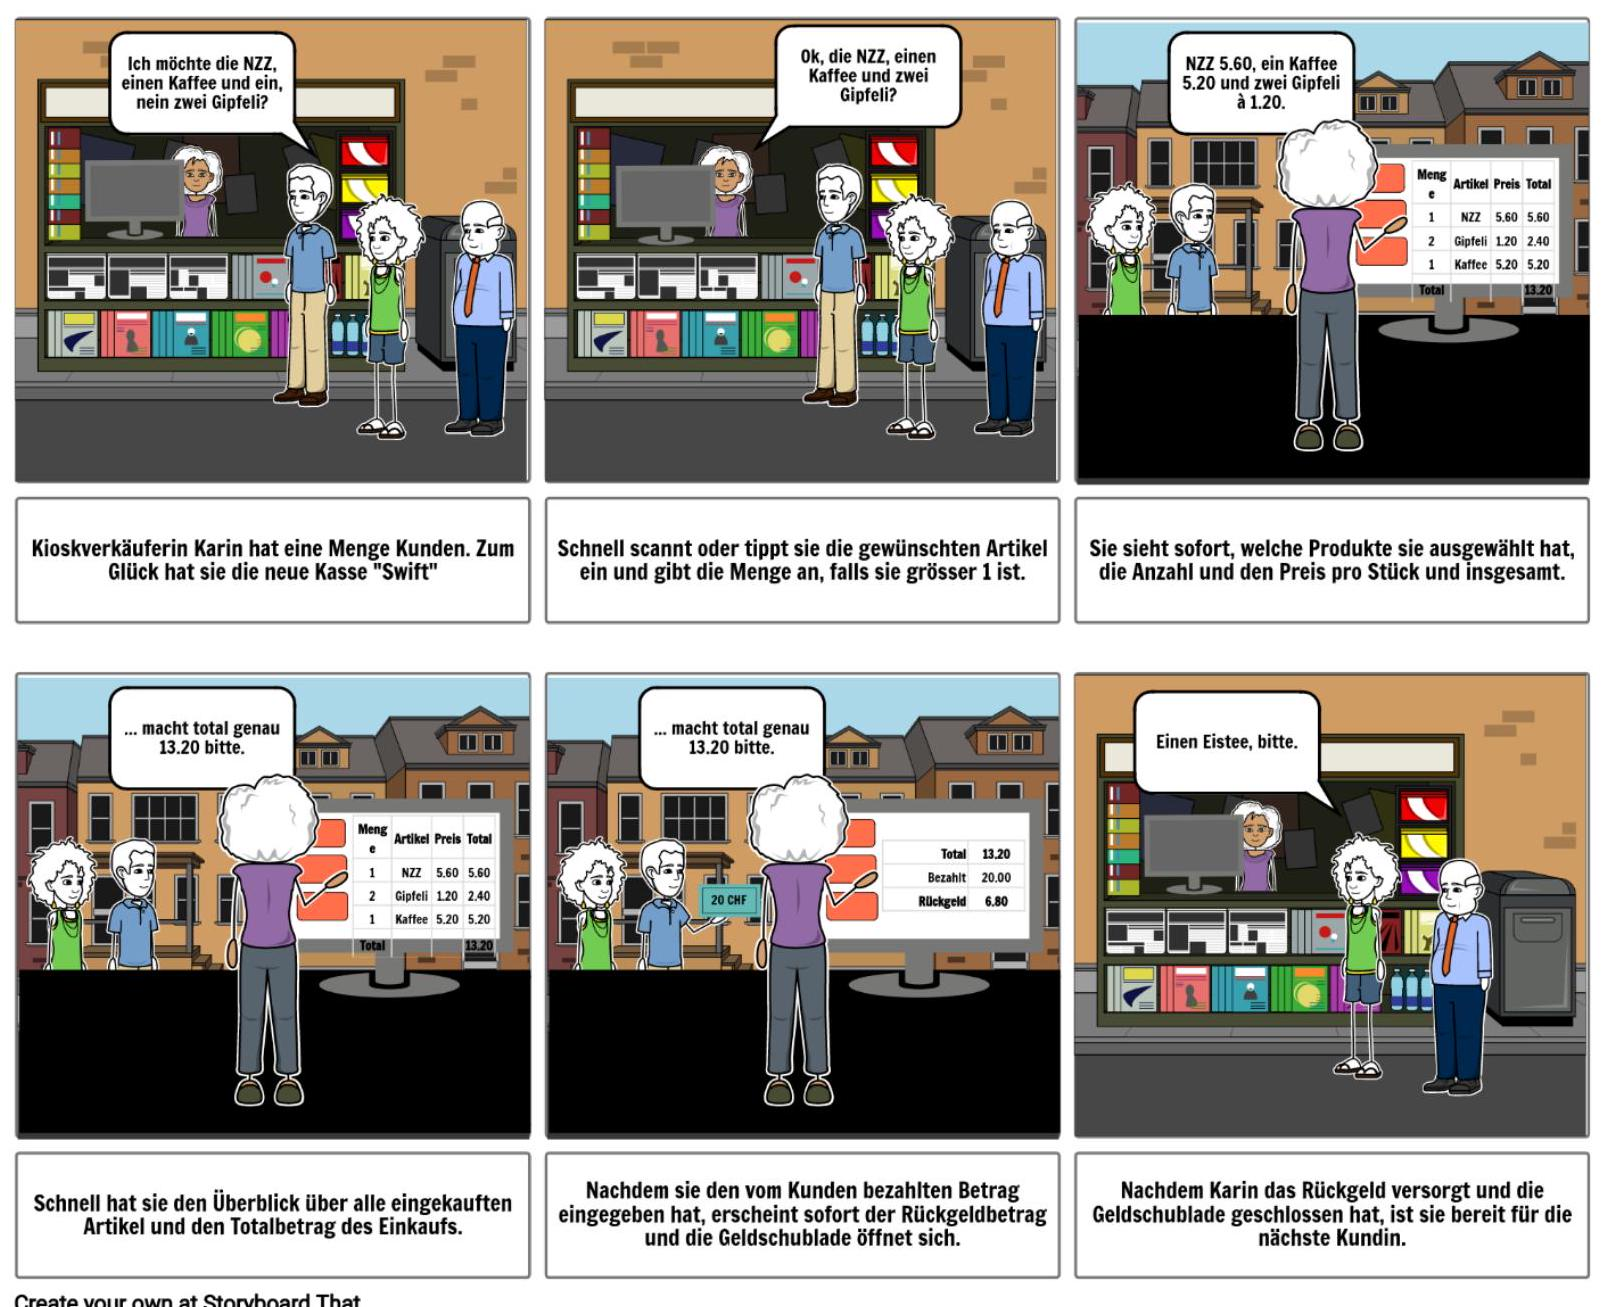
\includegraphics[max width=\textwidth, center]{2025_01_02_6e0302462f81f53e08d0g-23}
\end{itemize}

\begin{enumerate}
  \item Was ist Usability
  \item Was sind die wichtigsten Usability-Anforderungen
  \item Wie kann man diese Forderungen bei der Softwareentwicklung umsetzen
  \item Wrap-up und Ausblick
\end{enumerate}

\section*{Wrap Up (1/4)}
\begin{itemize}
  \item Usability
  \item Deutsch: Gebrauchstauglichkeit
  \item User Experience
  \item = Usability + Desirability
  \item Customer Experience
  \item = Usability + Desirability + Brand Experience
  \item Wichtigste 3 Usability-Ziele
  \item Effektivität
  \item Effizienz
  \item Zufriedenheit
  \item DIN EN ISO 9241-110:
\end{itemize}

7 wichtige Usability-Anforderungen

\begin{itemize}
  \item Aufgabenangemessenheit
  \item Lernförderlichkeit
  \item Individualisierbarkeit
  \item Erwartungskonformität
  \item Selbstbeschreibungsfähigkeit
  \item Steuerbarkeit
  \item Fehlertoleranz
\end{itemize}

\section*{- UCD-Prozess}
\begin{center}
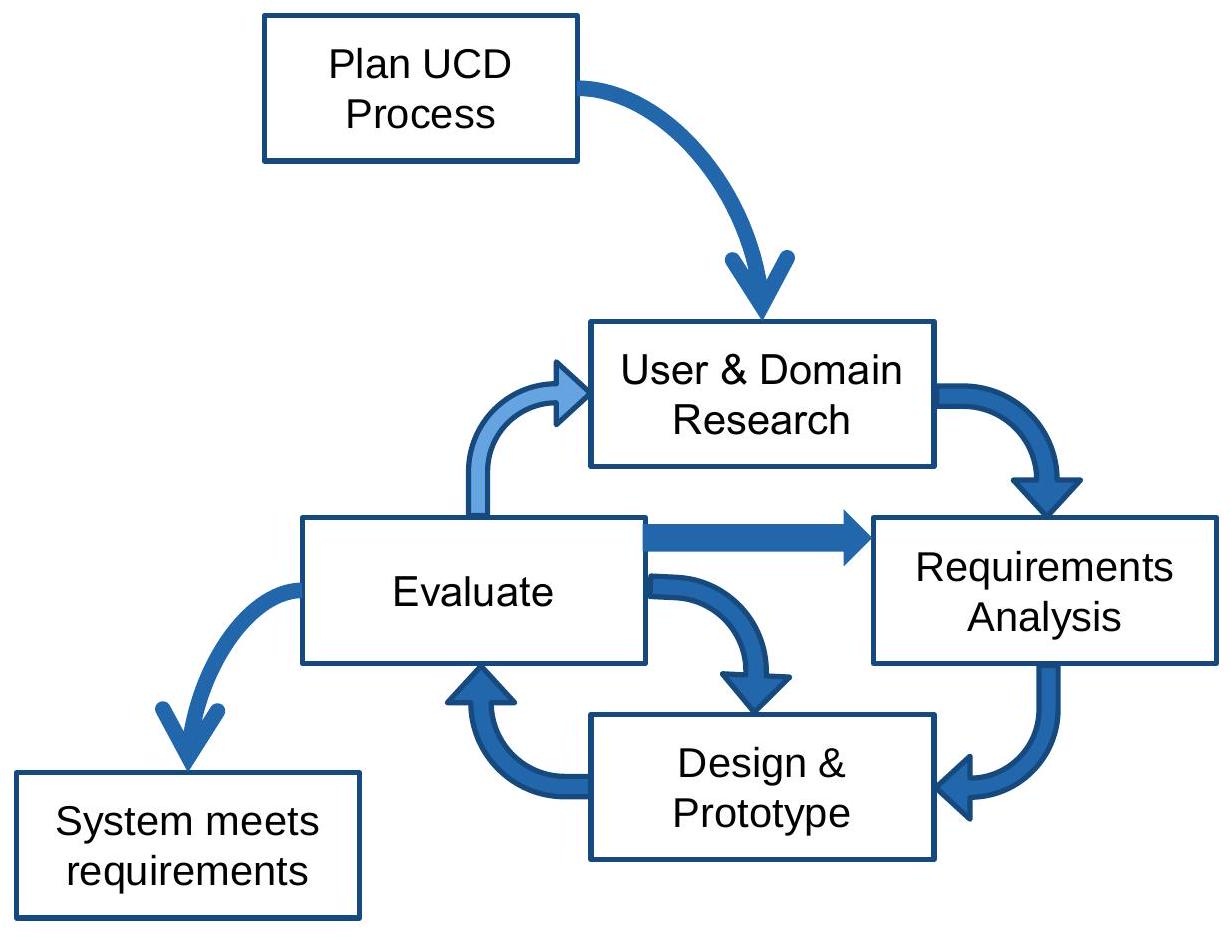
\includegraphics[max width=\textwidth]{2025_01_02_6e0302462f81f53e08d0g-26}
\end{center}

\begin{itemize}
  \item User \& Domain Research
  \item Wer sind die User
  \item Was sind ihre Ziele, ihr Kontext
  \item Was ist der Unternehmenskontext
  \item Requirements Analysis
  \item Wann, wie und warum interagiert der Benutzer mit dem System
  \item Was sind die wichtigsten Anforderungen an die Interaktion und das System aus Benutzersicht
\end{itemize}

\section*{Wrap Up (3/4)}
School of Engineering

\begin{itemize}
  \item UCD-Prozess\\
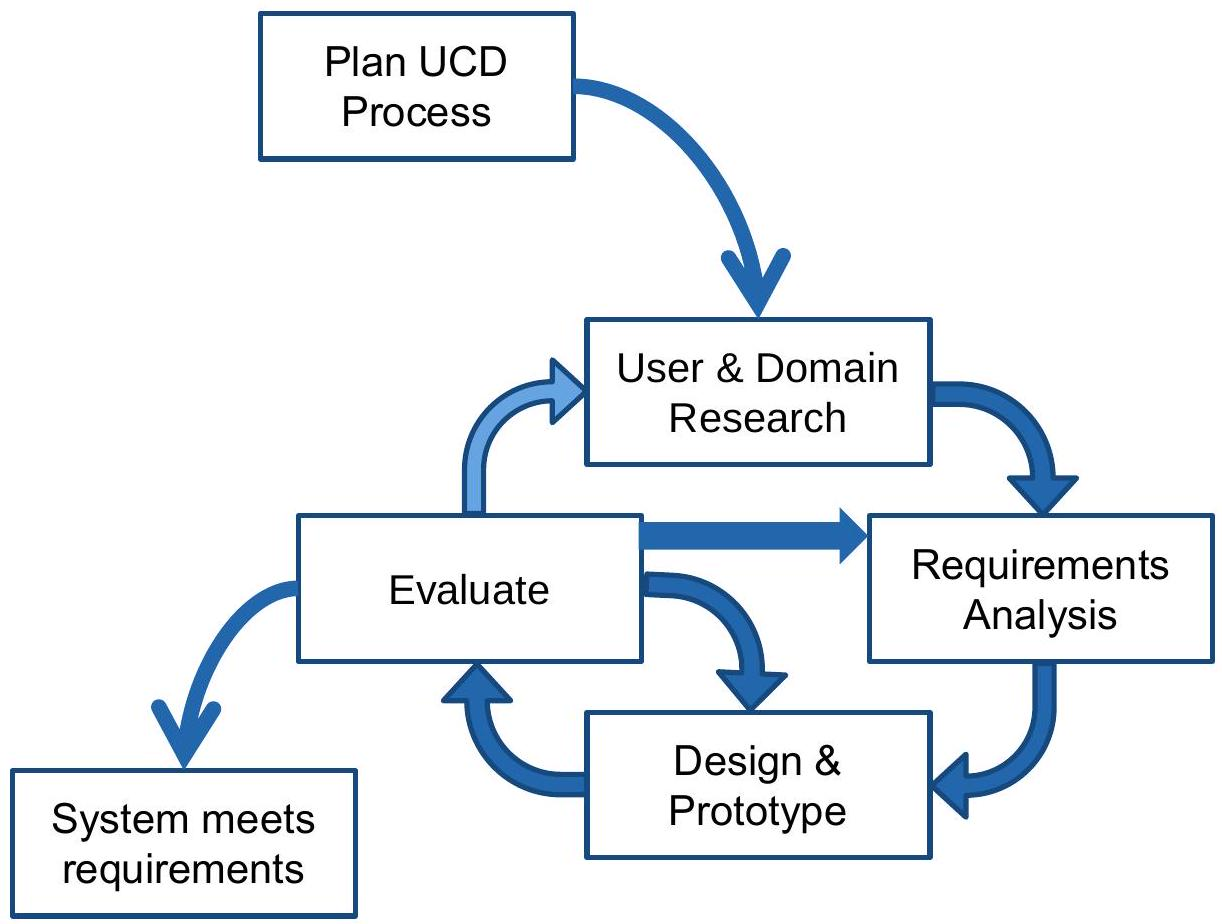
\includegraphics[max width=\textwidth, center]{2025_01_02_6e0302462f81f53e08d0g-27}
  \item Design \& Prototype
  \item Entwicklung des Interaktionskonzepts
  \item Umsetzung des Konzepts mit Interaktionsprototypen
  \item Evaluate
  \item Test des Interaktionskonzepts mit
  \item Benutzern
  \item Fachexperten
  \item Basierend auf den Interaktionsprototypen
\end{itemize}

\section*{Wrap Up (4/4)}
\section*{- UCD-Prozess}
\begin{center}
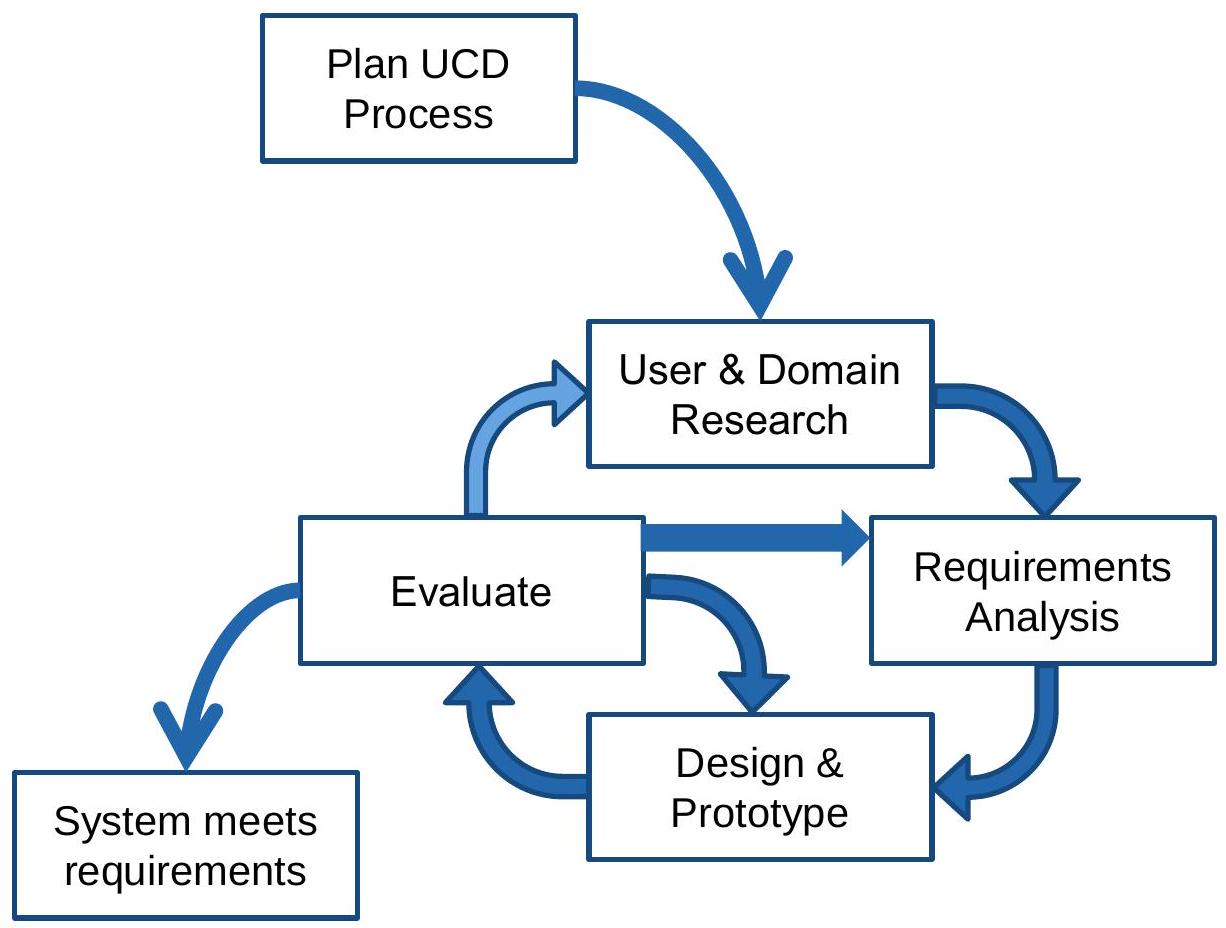
\includegraphics[max width=\textwidth]{2025_01_02_6e0302462f81f53e08d0g-28}
\end{center}

\begin{itemize}
  \item Wichtige Artefakte aus dem UCD
  \item Personas
  \item Usage-Szenarien
  \item Mentales Modell
  \item Stakeholder Map
  \item Service Blueprint / Geschäftsprozessmodell
  \item Storyboards
  \item Interaktionskonzepte
  \item Interaktionsprototypen (Wireframes)
  \item In der nächsten Lerneinheit werden wir die Frage beantworten:
  \item Wie bringt man UCD in Softwareentwicklungsprozesse ein?
\end{itemize}

\section*{Quellenverzeichnis}
[1] M. Richter and M. D. Flückiger, Usability und UX kompakt: Produkte für Menschen, 4th ed. Springer Vieweg, 2016.\\[0pt]
[2] Larman, C.: UML 2 und Patterns angewendet, mitp Professional, 2005\\[0pt]
[3] Seidel, M. et al.: UML @ Classroom: Eine Einführung in die objektorientierte Modellierung, dpunkt.verlag, 2012\\[0pt]
[4] Martin, R. C.: Clean Architecture: A Craftsman's Guide to Software Structure and Design, mitp Professional, 2018


\end{document}